\section{Aspectos Técnicos da Plataforma Brasil Participativo}

Nesta seção será abordada a maneira como foi desenvolvida a plataforma Brasil Participativo utilizando-se do \textit{framework Ruby on Rails} e da \textit{gem Decidim}. O objetivo dessa seção é elucidar como a plataforma foi inicialmente desenvolvida, o atual estado, e explorar em detalhes a \textit{gem Decidim}.

\subsection{Como foi Desenvolvida a Plataforma Brasil Participativo}

A plataforma Brasil Participativo foi desenvolvida com o \textit{framework Ruby on Rails} utilizando a \textit{gem Decidim}. Segundo a própria documentação disponibilizada pela comunidade de contribuidores do \textit{Decidim}, a \textit{gem} é descrita como um \textit{framework} que visa possibilitar que qualquer pessoa possa criar uma plataforma \textit{web} para ser utilizada como rede política para participação democrática. O Decidim fornece a organizações a capacidade de criar processos para planeamento estratégico, orçamento participativo, concepção colaborativa de regulamentos, espaços urbanos e processos eleitorais \cite{decidim-about}.

A plataforma no presente momento se apoia totalmente nas funcionalidades disponibilizadas pela \textit{gem Decidim}, preocupando-se apenas em implementar em sua instância correções de \textit{bugs}, customizações de estilo e comportamento de regras de negócio, e funcionalidades extras. De fato, a maior parte do código executado na plataforma não é visto em seu repositório oficial, pois este está abstraído dentro da \textit{gem Decidim}. O repositório oficial do Brasil Participativo está disponível no \textit{Gitlab} no endereço: \href{https://gitlab.com/lappis-unb/decidimbr/decidim-govbr}{https://gitlab.com/lappis-unb/decidimbr/decidim-govbr}. Já o repositório oficial do \textit{Decidim} está disponível no \textit{Github} no endereço: \href{https://github.com/decidim/decidim}{https://github.com/decidim/decidim}.


\subsection{Arquitetura do Decidim}

O Decidim possui várias entidades em sua arquitetura, mas as mais importantes para entendimento da regra de negócio são os espaços participativos e os componentes, referidos na documentação como \textit{participatory spaces} e \textit{components}, respectivamente. Uma visão macro das entidades do \textit{Decidim} pode ser visto na figura \ref{fig:arquitetura-decidim}. O \textit{Decidim} armazena dados de cada uma dessas estruturas utilizando a abordagem padrão de aplicações \textit{Rails like}, isto é, utilizando-se do \textit{Active Record} e persistindo os dados em um banco de dados relacional, o \textit{PostgreSQL}.

\begin{figure}[htbp]
  \centering
  \caption{Arquitetura do \textit{Decidim}}
  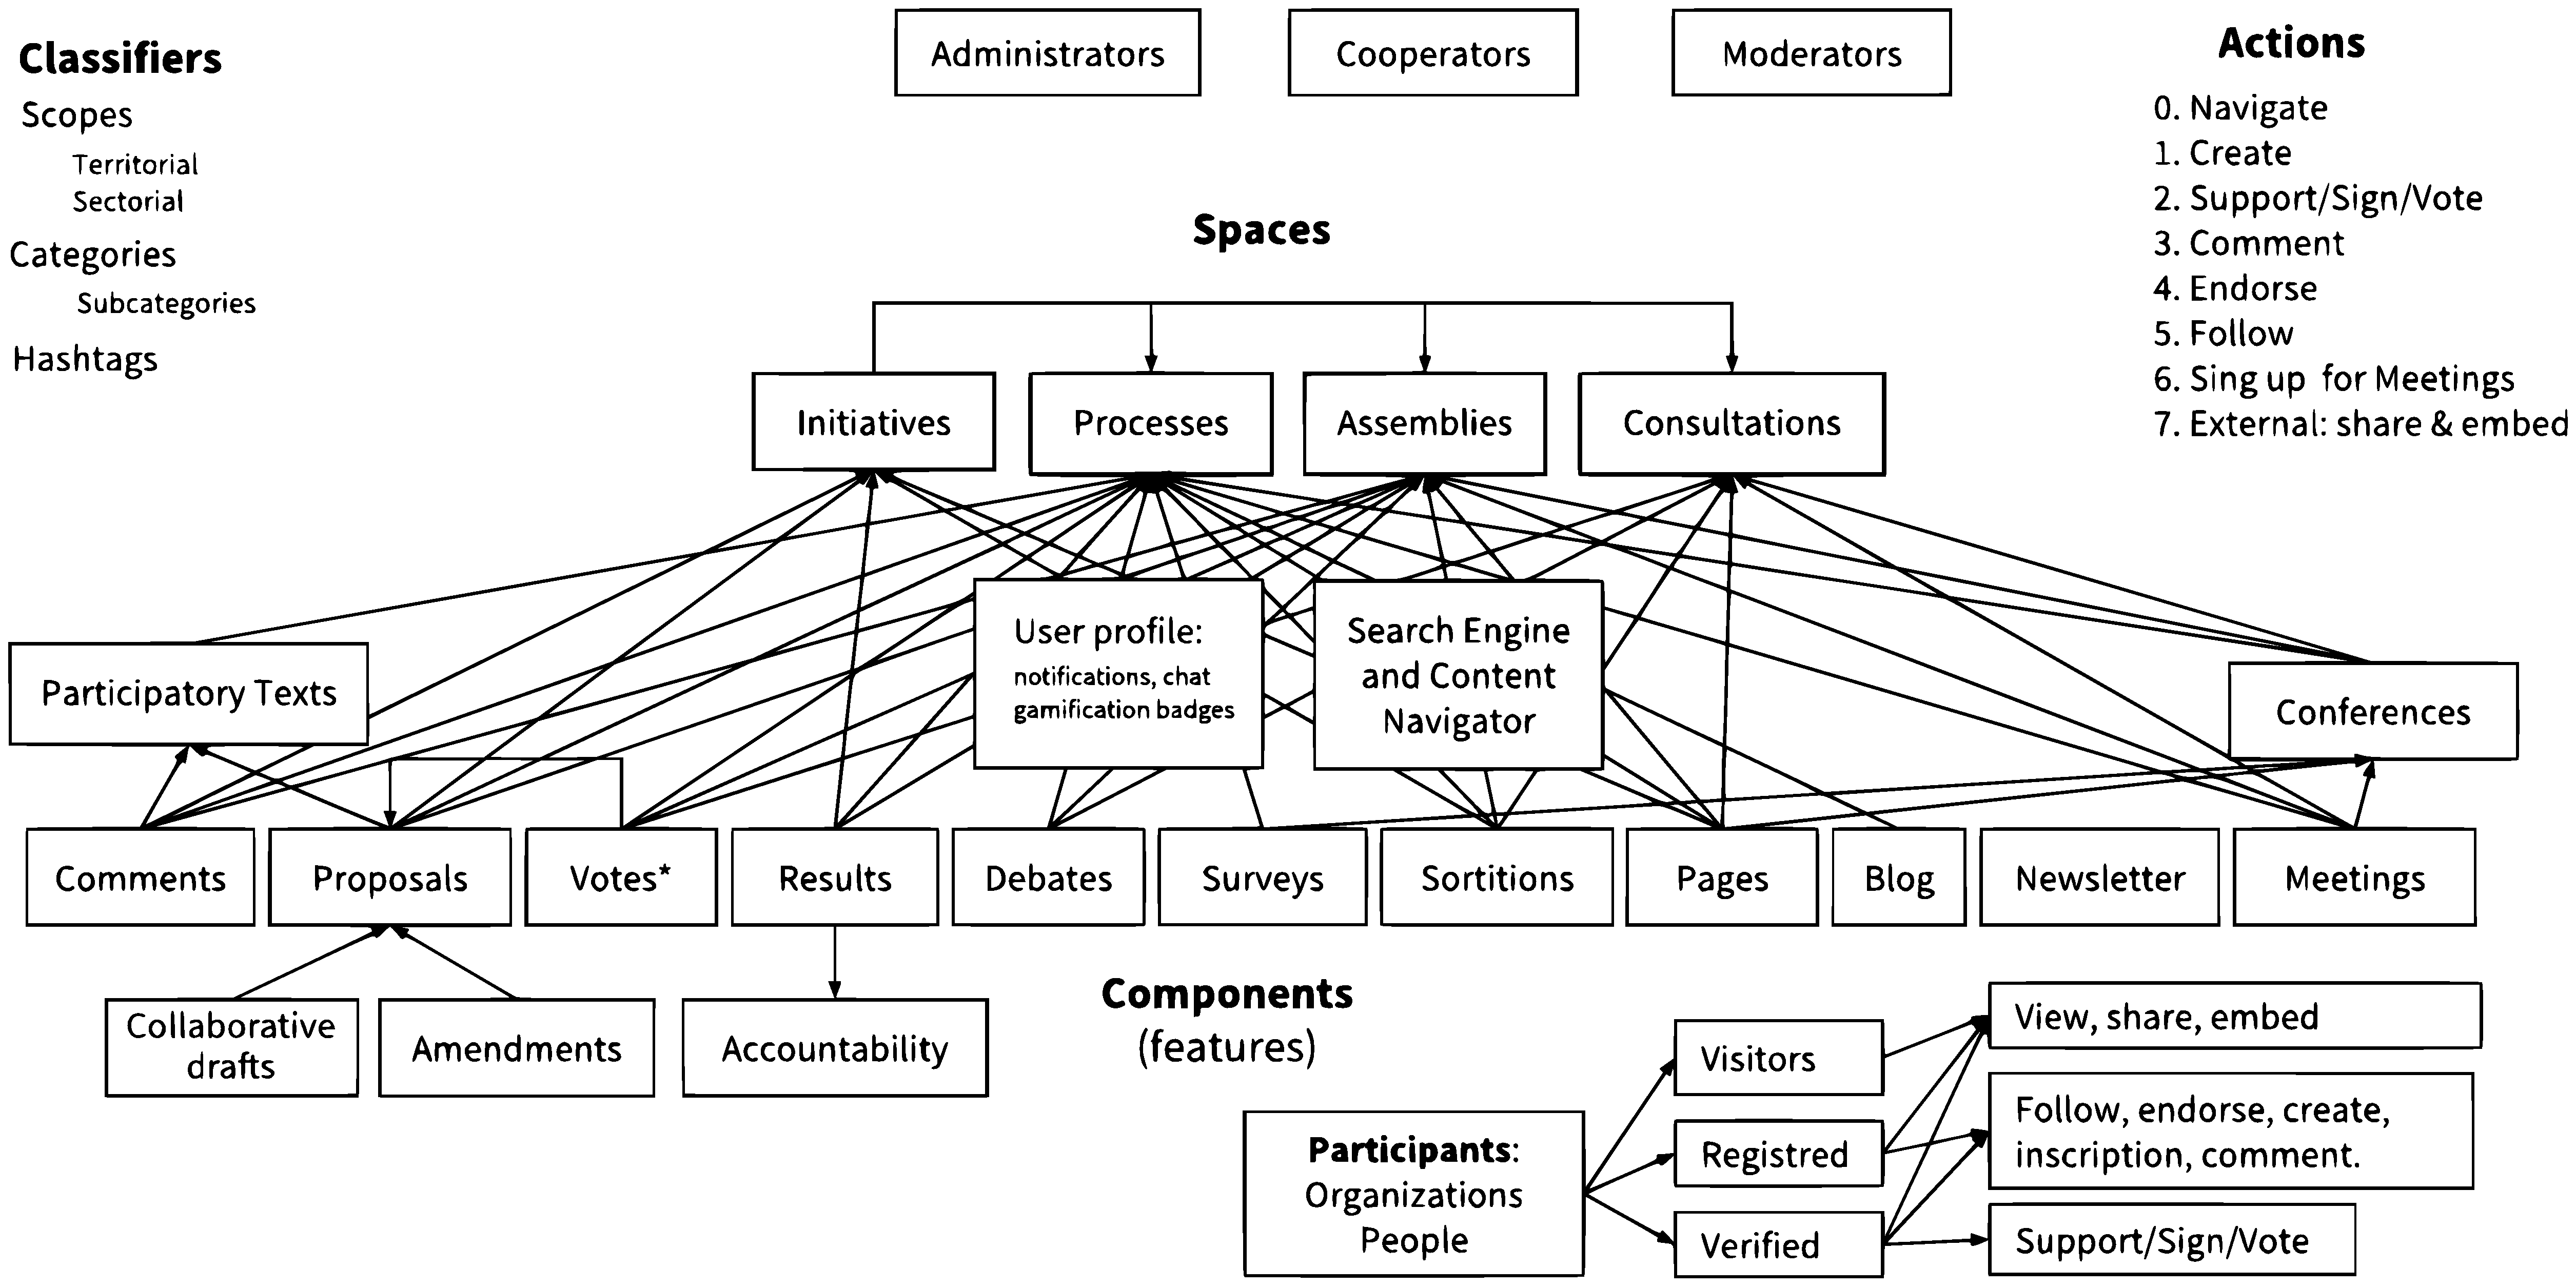
\includegraphics[width=\textwidth]{figuras/diagrama_decidim-min.eps}
  \fonte{Retirado de \cite{decidim-descriptionpage}}
  \label{fig:arquitetura-decidim}
\end{figure}

\subsubsection{Participatory Spaces}

Os \textit{participatory spaces} são \textit{frameworks} que definem como a participação será realizada, os canais ou meios pelos quais cidadãos ou membros de uma organização podem processar solicitações ou coordenar propostas e tomar decisões. Iniciativas, processos, assembleias e consultas são todos espaços participativos, estes referidos na documentação como \textit{initiatives}, \textit{participatory processes}, \textit{assemblies} e \textit{consultations}, respectivamente. Exemplos específicos incluem: uma iniciativa cidadã para alterar diretamente uma regulamentação; uma assembleia geral ou conselho de trabalhadores; um orçamento participativo, planejamento estratégico ou processo eleitoral; um referendo ou uma convocação para votar "Sim" ou "Não" para mudar o nome de uma organização \cite{decidim-descriptionpage}.

A nível de código, cada implementação de um novo \textit{participatory space} é feita em um sub-modulo separado em uma \textit{gem} própria. Uma relação entre cada um dos espaços participativos já existentes por padrão no \textit{Decidim} e o seu respectivo sub-modulo pode ser vista no quadro \ref{tab:modulos-participatoryspaces}

\begin{table}
  \centering
  \begin{tabular}{|c|c|c|}
    \hline
    Espaço Participativo & Módulo \\
    \hline
    Assembleias & decidim-assemblies \\
    Consultas ou Eleição & decidim-elections \\
    Iniciativas & decidim-initiatives \\
    Processos Participativos & decidim-participatory\_processes \\
    \hline
  \end{tabular}
  \caption{Módulos dos espaços participativos padrões do \textit{Decidim}}
  \label{tab:modulos-participatoryspaces}
\end{table}

\subsubsection{Components}

Os \textit{components} são os mecanismos participativos que permitem uma série de operações e interações entre os usuários da plataforma dentro de cada um dos espaços participativos. No \textit{Decidim} há disponível por exemplo os seguintes componentes: comentários, propostas, debates, pesquisas, sorteios, blogs e reuniões. Outros componentes que se baseiam nos componentes básicos são: textos participativos, responsabilidade e conferências \cite{decidim-descriptionpage}.

Da mesma forma que ocorre com os espaços participativos, os componentes são implementados através de sub-módulos em formato de novas \textit{gems}. No quadro \ref{tab:modulos-components} é possível conferir o nome do módulo de cada componente fornecido por padrão pelo \textit{Decidim}.

\begin{table}
  \centering
  \begin{tabular}{|c|c|c|}
    \hline
    Componente & Módulo \\
    \hline
    Comentários & decidim-comments \\
    Propostas & decidim-proposals \\
    Debates & decidim-debates \\
    Pesquisas & decidim-surveys \\
    Sorteios & decidim-sortitions \\
    \textit{Blogs} & decidim-blogs \\
    Reuniões & decidim-meetings \\
    \hline
  \end{tabular}
  \caption{Módulos dos espaços participativos padrões do \textit{Decidim}}
  \label{tab:modulos-components}
\end{table}

\section{}